\documentclass[11pt]{article}
\usepackage[margin=1in]{geometry}
\usepackage[T1]{fontenc}
\usepackage{lmodern}
\usepackage{microtype}
\usepackage{graphicx}
\usepackage{booktabs}
\usepackage{tabularx}
\usepackage{xcolor}
\usepackage{tikz}
\usetikzlibrary{arrows.meta,positioning,fit}
\usepackage[numbers,sort&compress]{natbib}
\usepackage[colorlinks=true,linkcolor=blue!50!black,citecolor=blue!50!black,urlcolor=blue!50!black]{hyperref}
\usepackage{caption}
\captionsetup{font=small,labelfont=bf}
\setlength{\parskip}{0.4em}
\setlength{\parindent}{0pt}

% Figures fall back to a labelled box if the file has not been copied into figures/ yet.
\newcommand{\figfile}[2]{\IfFileExists{figures/#1}{\includegraphics[width=#2]{figures/#1}}{%
  \fbox{\begin{minipage}[c][4cm][c]{#2}\centering\small Figure file not found: figures/\detokenize{#1}\par
  (copy it from paper/figures/ in the repo)\end{minipage}}}}

\title{\textbf{Dark Edges}\\[0.3em]
\large The Gemma~4 code graphs miss method calls, not functions,\\ and filling them in does not fix localisation}
\author{Soumi Sharma\\ Indian Institute of Science, Bengaluru}
\date{Gemma 4 Developer Agent: Paper Track, November 2026}

\begin{document}
\maketitle

\begin{abstract}
\noindent
The Gemma~4 Developer Agent competition gives every agent a precomputed code graph: a map of which function calls which. I wanted to know how much of what the code actually does at run time is missing from that map, and whether the missing part matters for finding the bug. I ran the failing tests of 103 tasks under a lightweight tracer and compared the calls that really happened with the released graphs. Between 47\% (fastapi) and 81\% (rich) of runtime call pairs have no edge in the graph. The reason is simple: calls \emph{into methods} are almost never in the graph (87--100\% missing), while calls into plain functions mostly are (12--17\% missing). Repositories differ only because some call methods more. The function that the real fix edits is executed by the failing tests in 81--83\% of tasks, but lies within three graph hops of the failure in only 24--26\%. A short static pass over the released node text recovers 41\% of the missing edges, yet it does not improve graph-based localisation. Finally, in a pre-registered test, giving a 4B Gemma agent a tracing tool did not help (gold file touched 0.60 vs 0.70 with graph tools), and the agent called the tool in only about a quarter of runs. My takeaway: the graph is incomplete in a predictable way, but the bigger gap for small agents is getting and using runtime evidence at all. Results cover four repositories and one model.
\end{abstract}

\section{Introduction: why look at the map?}

In this competition an agent based on Gemma~4 gets a GitHub issue and a repository snapshot, and has to produce a patch that makes hidden tests pass \citep{kaggle2026paper}. To help with navigation, the organisers released a \emph{code graph} for every task: each node is a function, method or class, and an edge $A \rightarrow B$ means ``$A$ calls $B$''. The agent queries it through tools such as \texttt{get\_code\_neighbors}, as in graph-guided systems like LocAgent \citep{chen2025locagent}.

Such a graph is built by reading the code without running it: a \emph{static} call graph. Python makes this hard: \texttt{self.render()} only tells you that \emph{some} method called \texttt{render} will run, and frameworks call your code through decorators and dispatch tables. So the question I started with was: \textbf{when a failing test runs, how many of the calls it makes are invisible in the graph, which ones, and does that hurt bug localisation?} I call a runtime call with no matching graph edge a \textbf{dark edge}.

This is not a new worry. A public audit ran each repository's whole test suite and found that the graphs hold only 14--21\% of runtime call pairs and none of 10{,}321 resolvable \texttt{self.m()} calls \citep{akhil2026audit}; others found no async functions at all \citep{aghasalim,forum745998} and rebuilt the graphs \citep{mindthemap,codegraphloc}. Outside the competition, DyPyBench found 51\% of dynamic Python call edges missing from PyCG's static graphs \citep{bouzenia2024dypybench}. I build on this and add:
\begin{enumerate}\setlength\itemsep{0.1em}
\item which calls go dark (methods vs functions), which explains the differences between repositories (Section~\ref{sec:dark});
\item how often the edit location is executed by the failing tests versus reachable in the graph, with an upper bound on what runtime evidence could buy (Section~\ref{sec:loc});
\item a cheap static repair that recovers 41\% of dark edges, and the finding that it does not help localisation (Section~\ref{sec:repair});
\item a pre-registered agent experiment with a tracing tool for Gemma~4 E4B, which came out null (Section~\ref{sec:agent}).
\end{enumerate}
My hypotheses (H1--H4) were frozen before any analysis, and I report the ones that failed.

\section{Setup}\label{sec:setup}

\begin{figure}[t]
\centering
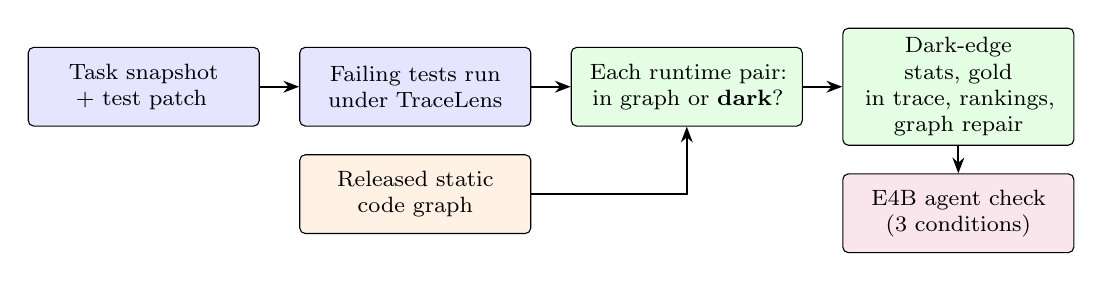
\begin{tikzpicture}[node distance=0.35cm and 0.5cm, every node/.style={font=\footnotesize},
  box/.style={draw, rounded corners=2pt, align=center, minimum height=1cm, text width=2.7cm, fill=#1!10}, box/.default=gray,
  arr/.style={-{Stealth[length=2mm]}, thick}]
\node[box=blue] (task) {Task snapshot\\+ test patch};
\node[box=blue, right=of task] (trace) {Failing tests run\\under TraceLens};
\node[box=green, right=of trace] (cmp) {Each runtime pair:\\in graph or \textbf{dark}?};
\node[box=green, right=of cmp] (out) {Dark-edge stats, gold\\in trace, rankings,\\graph repair};
\node[box=orange, below=of trace] (graph) {Released static\\code graph};
\node[box=purple, below=of out] (agent) {E4B agent check\\(3 conditions)};
\draw[arr] (task) -- (trace);
\draw[arr] (trace) -- (cmp);
\draw[arr] (graph) -| (cmp);
\draw[arr] (cmp) -- (out);
\draw[arr] (out) -- (agent);
\end{tikzpicture}
\caption{Pipeline. Tracing and comparison need only the standard library; the agent check uses the competition harness.}
\label{fig:pipeline}
\end{figure}

\textbf{Tasks.} The competition has 129 tasks from four repositories: fastapi (67), rich (48), requests (13) and httpx (1). For each task I ran the test files touched by the test patch twice: on the base snapshot plus test patch (``pre''), and with the gold fix added (``post''). A task is \emph{valid} if at least one test fails in pre and none fail in post. About a quarter of the tasks needed small stand-ins for two test-only packages missing from the offline package store. 103 tasks were valid (fastapi 58, rich 39, requests 5, httpx 1). A looser set of 120 tasks is my sensitivity check; every headline holds on both. With so few requests and httpx tasks, I make no per-repository claims about them.

\textbf{Tracer.} TraceLens is a small tracer (about 260 lines, standard library only) that uses Python's \texttt{sys.monitoring} hook to record every call between functions of the repository, per test. When the call passes through library code (for example a web framework calling your route handler), it links the nearest repository caller to the callee and marks the edge as \emph{lifted}. Overhead on these tests was 0.9--1.3$\times$, and all 129 tasks traced in a single CPU notebook session.

\textbf{Dark edges.} I map traced functions to graph node ids (module path plus qualified name); for fastapi 93\% of call volume maps; the rest is mostly async methods, which the graph does not contain. A \emph{dark edge} is a runtime pair (caller, callee), both in the graph, with no \texttt{calls} edge between them. I count unique pairs per task and average over tasks within a repository.

\textbf{Gold location.} The ``gold'' functions are those whose lines the real fix changes. 89 of the 103 valid tasks have at least one gold function in the graph; the rest edit code outside functions or in functions the graph lacks.

\textbf{Statistics.} Confidence intervals (CIs) are 95\% percentile intervals from a \emph{task-clustered bootstrap}: I resample whole tasks 10{,}000 times, so pairs from the same task stay together. Paired yes/no comparisons use the exact McNemar test, which looks only at the cases where two methods disagree.

\textbf{Pre-registration.} Before the analysis I committed four hypotheses: H1, fastapi has the most dark edges and requests the fewest; H2, trace-based ranking beats a static two-hop neighbourhood by at least 10 points of recall@20; H3, the released embeddings do not predict dark edges better than a name-similarity baseline; H4, a tracing tool raises how often a small agent's patch touches a gold file. Every analysis decided after seeing data is labelled \emph{exploratory} below.

\section{Which calls go dark?}\label{sec:dark}

\begin{table}[t]
\centering\small
\begin{tabular}{lccc}
\toprule
 & fastapi (58 tasks) & requests (5) & rich (39) \\
\midrule
All runtime pairs (headline) & 0.47 [0.44, 0.51] & 0.52 [0.44, 0.59] & 0.81 [0.75, 0.84] \\
\quad callee is a module-level function & 0.14 (66\% of pairs) & 0.12 (52\%) & 0.17 (12\%) \\
\quad callee is a method of the same class & 1.00 (8\%) & 1.00 (22\%) & 1.00 (44\%) \\
\quad callee is a method of another class & 1.00 (25\%) & 1.00 (26\%) & 0.87 (45\%) \\
\bottomrule
\end{tabular}
\caption{Share of runtime call pairs that are dark (no graph edge), by type of callee. Brackets: 95\% CI. Percentages: share of that repository's pairs.}
\label{tab:dark}
\end{table}

\begin{figure}[t]
\centering
\figfile{F5_callee_type.png}{0.7\linewidth}
\caption{Dark fraction by callee type. Methods are almost always dark; plain functions mostly are not.}
\label{fig:callee}
\end{figure}

Over all 103 tasks there are 14{,}059 unique runtime pairs and 10{,}067 of them (72\%) are dark. Per repository, Table~\ref{tab:dark} shows the pattern that explains almost everything: \textbf{a call into a module-level function is usually in the graph, and a call into a method almost never is}. In these graphs a method's calls are mostly attached to its class node instead (68--95\% of all \texttt{calls} edges touch a class node).

This also explains the differences between repositories. Rich looks ``darker'' because 88\% of its executed calls go into methods, against 48\% for requests and 34\% for fastapi. Across tasks, the share of method callees and the dark fraction correlate at $r = 0.94$. This is partly built in, so it confirms the composition story rather than adding independent evidence. \textbf{H1 is not supported}: the order is rich $>$ requests $>$ fastapi, and rich exceeds fastapi by 0.33 with a CI that excludes zero.

\textbf{Reconciling with the public audit (exploratory).} Pooled over pairs, rich is 84\% dark, matching the audit's 79--86\%; fastapi is 43\% (37\% without framework dispatch, which the audit also leaves out). I trace only each task's own test files, which in fastapi mostly call plain functions, while the audit runs whole suites. A second view confirms the mechanism: if a call counts as covered whenever the graph links the caller to the \emph{callee's class} (two hops via the class node), all three repositories drop to 24--28\% dark. The graph knows which class is involved, not which method.

\section{Does the missing part matter for localisation?}\label{sec:loc}

\textbf{Is the bug where the tests run?} In 83\% of the 89 ranked tasks (81\% on the looser set), the gold function is executed by the failing tests. In 29\% it is executed \emph{only} by failing tests and never by passing ones, and in 20\% it is reached at run time only through dark edges. But only 24\% of gold functions lie within three graph hops of the function where the test failed, even with class nodes allowed as stepping stones. So the run-time path to the bug exists most of the time, and the graph usually does not show it.

\begin{table}[t]
\centering\small
\begin{tabular}{lcc}
\toprule
Ranking method (recall@20) & strict, 89 tasks & loose, 104 tasks \\
\midrule
Ochiai over failing vs passing tests (oracle) & 0.63 [0.54, 0.72] & 0.59 \\
Distance from the failure in the runtime call graph (oracle) & 0.57 [0.47, 0.67] & 0.53 \\
BM25 text search, issue vs function source & 0.46 [0.36, 0.56] & 0.48 \\
Static graph, two hops from symbols named in the issue & 0.26 [0.18, 0.35] & 0.27 \\
\bottomrule
\end{tabular}
\caption{How often a gold function is in the top 20 of each ranking. ``Oracle'' methods use the tests that define the task, which an agent does not have, so they are upper bounds.}
\label{tab:rank}
\end{table}

\textbf{How much could runtime evidence help?} I ranked all graph functions for each task in four ways and asked whether a gold function is in the top $K$ (recall@$K$; ties are broken randomly and averaged over 100 shuffles). The first is \emph{Ochiai}, a classic spectrum-based fault-localisation score \citep{abreu2007ochiai,wong2016survey}: a function scores high if many failing tests and few passing tests run it. The second ranks functions by distance from the failure in the runtime graph. The third is BM25 text search (issue vs function source); the last, functions within two graph hops of symbols named in the issue.

Table~\ref{tab:rank} shows the result. Ochiai beats the static baseline by 37 points (CI 26 to 49, McNemar $p < 0.001$), so \textbf{H2 is supported}. Both runtime rankings use the hidden failing tests: they show what runtime evidence \emph{could} carry, not what an agent achieves. Also, 26 of the 89 issues name no graph symbol, so the static baseline gets nothing there, and Ochiai's lead over BM25 is not stable across task sets.

\textbf{Can the graph's embeddings predict dark edges?} The competition also ships a 256-dimensional embedding per node. Using held-out repositories, embedding similarity separates dark edges from random non-edges better than name similarity (AUC 0.70 vs 0.58 on fastapi, 0.70 vs 0.55 on rich; AUC is the chance that a true edge scores above a non-edge). So \textbf{H3 is not supported}: the embeddings carry some call information, but the best models stay at AUC 0.68--0.74, consistent with the near-collapsed embeddings reported on the forum \citep{forum744040}.

\section{Can the graph be repaired cheaply? (exploratory)}\label{sec:repair}

Since most dark edges are method calls, I tried the obvious fix. I parsed the source text stored in each graph node and added three kinds of edges: (R1) \texttt{self.m()} or \texttt{cls.m()} inside a method, resolved to that class or its base classes; (R2) \texttt{self.m} used without a call, which covers properties; (R3) \texttt{X(...)}, resolved to \texttt{X.\_\_init\_\_}. It needs no execution.

\begin{figure}[t]
\centering
\figfile{F7_repair.png}{0.72\linewidth}
\caption{Dark fraction as repair rules are added (task mean, 95\% CI). Rules are cumulative.}
\label{fig:repair}
\end{figure}

The repair recovers 4{,}160 of the 10{,}067 dark pairs (41\%): 74\% of same-class method calls, but only 15\% of calls into other classes, all through constructors. Calls like \texttt{self.console.print()} need the type of \texttt{self.console}, which a text pass cannot see; tools such as PyCG or Jarvis \citep{salis2021pycg,huang2024jarvis} target this. As a precision check, of the added edges whose two endpoints both ran, 87\% were observed at run time. After repair, rich drops from 0.81 to 0.45 dark and fastapi from 0.47 to 0.34 (Figure~\ref{fig:repair}); pooled, the graph then holds 58\% of runtime pairs, close to the 62--69\% of the audit's full \texttt{ast} rebuild \citep{akhil2026audit}.

The surprising part is that the repaired graph \textbf{does not improve static localisation}: recall@20 for the two-hop baseline moves from 0.26 to 0.27 (CI of the change $-0.01$ to $+0.03$). Class nodes already connect sibling methods within two hops, so the new edges add little reachability. The bottleneck is elsewhere: a starting point in the issue text, and a path that only running the code reveals.

\section{Does a tracing tool help a small agent? (H4)}\label{sec:agent}

\textbf{Design.} I ran the competition harness with Gemma~4 E4B on 30 of the 89 ranked tasks (16 fastapi, 11 rich, 3 requests; stratified, seed 0) in three conditions: no graph tools; the three built-in graph tools; graph tools plus TraceLens. The prompt was identical (reproduce, localise, fix, verify, submit) except for the localisation step; in the tracer condition it told the agent to trace its reproduction script. Two sampling seeds, frozen budget of 10 minutes and 50 tool calls. The pre-registered outcome: does the patch touch a file the gold patch changes?

\begin{table}[t]
\centering\small
\begin{tabular}{lccc}
\toprule
 & No graph tools & Graph tools & Graph tools + tracer \\
\midrule
Gold file touched, all 180 runs & 0.72 & 0.70 & 0.60 \\
Resolved (hidden tests pass), all 180 runs & 0.18 & 0.18 & 0.13 \\
Gold file touched, 20 tasks with paired records & 0.70 & 0.70 & 0.70 \\
Mean tool calls / seconds per run & 12.1 / 165 & 14.0 / 206 & 14.8 / 204 \\
\bottomrule
\end{tabular}
\caption{Agent check with Gemma 4 E4B, 30 tasks, 2 seeds. Paired difference, tracer vs graph tools (recovered records): $-0.07$ [$-0.27$, $+0.10$], McNemar $p = 1$.}
\label{tab:agent}
\end{table}

\textbf{Result.} The tracer did not help: \textbf{H4 is not supported} (Table~\ref{tab:agent}). The graph tools did not help either, compared with no graph at all. The most telling number is uptake: the tracer's output reached the agent in only 9 of 32 recovered tracer runs (28\%), even though the prompt asked for it first. Runs that did trace hit a gold file about as often as runs that did not (0.67 vs 0.65). This fits other findings: agents used an available debugger in only 0.2--6.2\% of runs \citep{daxerer2026debugger}, small agents rarely chain graph queries \citep{bellam2026small}, and another entrant saw E4B call a map tool in 1 of 84 runs \citep{whoreads}. On the other side, one team reports more passes with graph tools for E2B over a larger sample \citep{nakrani}, and Debug2Fix \citep{garg2026debug2fix} gains by wrapping debugging in a sub-agent. So my null is about this tool design, model and sample size, not runtime evidence in general.

\textbf{A disclosure.} A notebook cell was re-executed while an earlier worker thread was still running, so part of the run had eight tasks in parallel instead of four, and the per-run file was lost with the session. The 180-run summary survived, and 92 per-run records (20 tasks with all three conditions at seed 0) were recovered from the printed log. Run times (165--206 s) stayed far below the 10-minute limit. This is logged in the amendment file.

\section{Related work}

The competition follows SWE-bench \citep{jimenez2024swebench}; SWE-agent \citep{yang2024sweagent} and Agentless \citep{xia2025agentless} showed how much the tool interface and pipeline matter. LocAgent, RepoGraph and CodexGraph \citep{chen2025locagent,ouyang2025repograph,liu2025codexgraph} give models graph views of a repository; my results suggest checking which edge types such graphs contain. Spectrum-based fault localisation is decades old \citep{abreu2007ochiai,wong2016survey}, and AutoCodeRover \citep{zhang2024autocoderover} already feeds it to an LLM agent. PyCG and Jarvis \citep{salis2021pycg,huang2024jarvis} build better static Python call graphs, and DyPyBench \citep{bouzenia2024dypybench} measures what they miss. Within the competition, the audits cited in Section~1 \citep{akhil2026audit,countzero,mindthemap,codegraphloc,graphnav} found the coverage gap and that fixes sit far from issue mentions; my additions are the method/function decomposition, the gap between execution and reachability from the failing frame, the oracle ceiling, the repair measured against runtime truth, and the agent test.

\section{Limitations}

Four repositories, two of which dominate (rich holds 70\% of pairs); one tracer configuration; 26 tasks I could not build; nested and async functions never map (the hosts state that no private task touches async code \citep{forum745998}). The ranking upper bounds use hidden tests. The agent check has 30 tasks, one model, one prompt and partially recovered records. Holm correction across H1--H4 changes nothing: H2 ($p < 0.001$) survives and the others were not supported.

\section{Conclusion and resources}

The released graphs miss most method calls, and that one pattern explains why some repositories look darker than others. The edit location is usually on the failing test's runtime path but not near it in the graph. Adding method edges is easy but does not make graph search find bugs, and a tracer does not help a 4B agent that rarely calls it. For the next agent I would make runtime evidence arrive automatically (trace the reproduction before the agent starts) rather than build a denser graph.

\textbf{Code and data.} TraceLens, the agent skill, all analysis scripts, the frozen protocol (\texttt{configs/protocol.yaml}, tag \texttt{protocol-v1}), the amendment log, and aggregate result tables are at \citep{darkedgesrepo}. Competition data and per-task traces are not redistributed, in line with the rules. Software: Python 3.12, seed 0, 100 tie-break shuffles, 10{,}000 bootstrap resamples.

\textbf{AI assistance.} I used an AI assistant to help write analysis code and to help draft and edit this text. The study design, experiments, numbers and conclusions are mine and were checked against the logged outputs.

\small
\bibliographystyle{unsrtnat}
\bibliography{refs}

\end{document}
